\chapter{Design}
This chapter describes the design decisions taken for the implementation of the Bazo Wallet. Section \ref{designguidelines} introduces design guidelines that were given from the start of the project. Section \ref{transactioninfo} and \ref{communication} explain how the required functionality of the Wallet was designed.
\section{Design Guidelines}\label{designguidelines}
For the development of the Bazo Wallet, multiple requirements were explored with the financial service provider. These are described in \ref{functionalreq}. This section introduces several design guidelines which were known from the start of the project and consequences on other design desicions.
\subsection{Progressive Web Applications}
The Bazo Wallet is supposed to be designed as a Progressive Web Application. Due to Progressive Web Applications having native elements, they provide a unified solution for multiple operating systems, targeting both mobile and desktop devices. This implies that a web application is to be crafted, that supports all the functional requirements described i \ref{functionalreq}. The Web application therefore needs to contain the following pages to support the core requirements:
\begin{itemize}
\item Page to share transaction data
\item Page to send new transactions
\item Page to inspect account state
\item Page to request new funds from bonus points
\end{itemize}

\subsection{Network Communication and Interfaces}
Since the Application is designed as a PWA and a quality requirement is the fully client side approach to all the operations, all operations need to be made in the browser. Since no backend application should be leveraged, the Web app needs to be able to sign transactions in the browser. All further communication with the Bazo network needs to be done over web interfaces. This led to the design of a RESTful web interface for the bazo light client, which was then implemented. The following operations should be supported by the API:
\begin{itemize}
\item Querying account state
\item Preparing transactions
\item Distributing transactions in the peer-to-peer network
\end{itemize}
\subsection{Device Sharing}
In order to explore how suitable a PWA approach to the implementation of a Wallet or payment application is, the application is required to share transaction data on a device-to-device basis. Technologies such as NFC and Bluetooth Low Energy should be evaluated for their browser support and implemented. 
The data model and mechanism applied to use the described technologies are explained in the consecutive sections.
%??%
\section{Transaction Information} \label{transactioninfo}
One requirement, that is that Bazo coins can be exchanged between users without direct involvement or administration from the service provider was incorporated into the core design of the Bazo currency. To fulfill said requirement it is vital that transaction informations can be shared between users of the Bazo Wallet. This section outlines how transaction information can be shared with the Bazo Wallet.
%Search for papers, resources etc.
Sharing transaction information in native applications is often achieved with technologies such as NFC, Bluetooth or by encoding and reading transaction information from a Quick-Response Code.
\subsection{Schema}\label{schema}
In order to communicate Bazo Transactions to other devices and applications, an URI Scheme was designed to hold transaction information, so that a requesting party can communicate it. The grammar and structure for the schema followed the \cite{bip21} 21st Bitcoin Improvement Proposal for an URI scheme since it contained all necessary elements to fulfill the requirement. The URI Schema consists of a required part which holds the protocol name and the recipient's fully qualified bazo address.


\[
\underbrace{\overbrace{bazo:}^{\mathrm{protocol}}\overbrace{34ad8...8a4a4}^{\mathrm{bazo address}}}_{\mathrm{required components}}
\underbrace{\overbrace{?amount=123}^{\mathrm{amoun t}}\overbrace{?label=1 Coffee}^{\mathrm{label}}\overbrace{?message=Message}^{\mathrm{message}}}_{\mathrm{optional components}}
\]


% reference nfc bridge
This implies, that the Bazo Wallet and other applications that need to interact with it need to be able to encode and decode transaction information as supplied in the described grammar.
For the web-based wallet this transaction info should also be an optional parameter of the URL of the payment page. This allows that a complete URI to the payment page with all required transaction information can be shared among users or between merchants and users.
This enables to encode complete transaction information as well as a an URI to the application page with the transaction information into media such as a QR-Code. This has the benefit, that all users of the Wallet can exchange payment information without having to know about the Schema.
Since merchants frequently have more advanced payment systems and don't want to encode payment information into media such as QR-Codes for each new transaction, the payment page of the Wallet also needs to be able to accept additional parameters, by which the Wallet can then query the transaction amount from a service.
The schema below shows the URI endpoint of the payment page, together with additional parameters that can be supplied to have the payment page prefilled with transaction information. This procedure is further described in Figure\ref{fig:POS}.
\[
\underbrace{\overbrace{https://host/:}^{\mathrm{Host}}\overbrace{/auth/user/send}^{\mathrm{payment page}}}_{\mathrm{required components}}
\underbrace{\overbrace{posid=323}^{\mathrm{POS identification}}\overbrace{?paymentinfo=bazo://123123}^{\mathrm{transaction info}}}_{\mathrm{optional components}}
\]

The implementation of the module to encode and decode bazo encoded transaction information is described in \cite{undefined}.
%reference impl

\subsection{Device Sharing}\label{pocnfcbridge}
In order to explore further possibilities on how to extend the browser support for native API's a Proof of Concept was designed. The PoC was targeted to the android Platform, since NFC support is still fairly limited on iOS devices at the time of the design. This means that with Core NFC, a technology by Apple, only communication with passive NFC Tags is supported \cite{corenfc}. The PoC, further referenced as 'NFC Bridge', should run as a background service and enable two processes.
\begin{enumerate}
\item Reading NFC devices:
The application should be registered as a handler for NFC messages. If an NFC message is read from another NFC device such as another active device or an NFC Tag, the user is prompted with applications that can handle the data format. If the user selects the NFC Bridge application, the data received from the NFC Adapter should be parsed and the user prompted with the Payment page of the Bazo Wallet. The payment page is then prefilled with the payment information extracted from the NDEF message.
\item Pushing to NFC devices: The NFC Bridge application should allow the PWA-based Bazo Wallet to push handover encoded transaction information which can then be pushed to NFC devices and tags.
The first design sketch included that communication between the Bridge application and the Bazo Wallet is done through an HTTP or Websocket. This implied that the NFC Bridge is running as a background service, listening for NFC messages and keeping the server alive.
Since the android platform allows starting the application when an NFC message is received through the configuration of application intents, this design was preferred.
\end{enumerate}

\subsection{Merchant options}\label{merchantoptions}
In order to completely support the payment process, which does require interaction of the application with backend services from the financial service provider, interfaces need to be integrated into the application.
This is also necessary since some platform do not support WebNFC in the browser, which means that the payment process can not be carried out in a complete device-to-device manner. On iOS devices support for NFC access is restricted to native API's and the functionality is limited to reading passive NFC Tags.
In order to get the complete payment process depicted, the payment process that is to be developed can be described as follows. The user of an iOS device can use his any NFC Tag Reader app from the app store. Before the payment process can be started, the merchant needs to supply payment information in form of a correct bazo address as well as some token that represents the Point-of-sale system. The merchant should have the possibility to write these informations to the NFC Tag at the POS, using the Mobile Wallet application.
Once this set up is in place, the user will approach the POS System and may start the payment process. The cashier will scan the items, and the POS System will automatically associate the POS ID with the transaction amount. The user can now use any existing iOS or android application to read the NFC tag. Since both payment and transaction information is encoded in a URL, the user is taken to the payment page of the Mobile Wallet, where the POS ID is used to query the transaction amount from the POS System. Since the Bazo Address is supplied in the URL as well, the user can confirm the payment. Once confirmed the Mobile Wallet will sign the transaction and send it into the Bazo network. Figure
\ref{fig:POS} shows the process of transferring transaction information and transaction issueing under the constraint that a third party service needs to be queried.

\begin{figure}
\centering
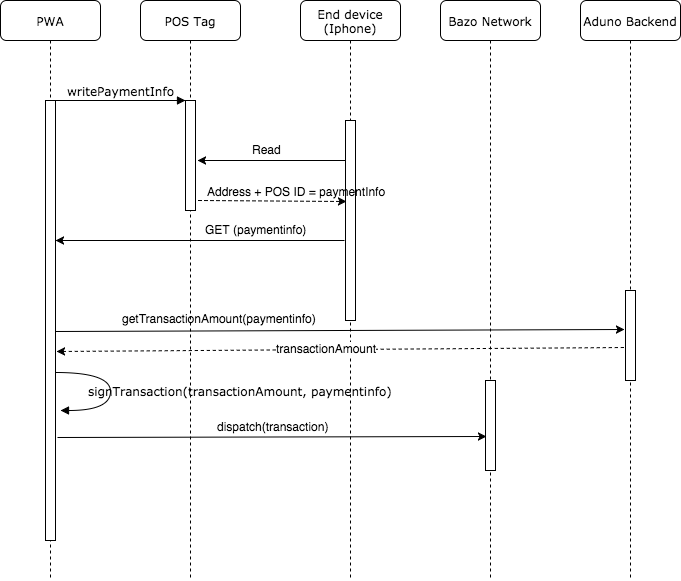
\includegraphics[width=1\textwidth]{diagrams/POS_flow.png}
\caption{\label{fig:POS}Transferring payment information across devices using NFC.}
\end{figure}

\section{Communication}\label{communication}
%% Interfaces includes integration of existing services
\subsection{Bazo Interfaces}
\subsection{Payment System Interfaces}

\subsection{Security Considerations}







\chapter{Implementation}
Chapter \cite{undefined} explained the design of the Bazo Wallet in order to fulfill the requirements to such an application captured in chapter \cite{undefined}. This chapter documents the implementation phase of the application. Chapter  \ref{architecture} outlines the architecture, the application employed. The following sections explain how the individual functional requirements were implemented.
\section{Architecture\label{architecture}}
The application was implemented as a Progressive Web Application. The constraints to a progressive web application have been outlined in \cite{undefined}. The application was implemented as a web application with the addition of the following items to comply as a progressive web application:
\begin{itemize}
\item Manifest
A manifest is a JSON file that describes metadata of a web application such as links to icons for different screen sizes. It is further used to configure the progressive web application. For example, the name that will be displayed in the app drawer on the phone once the app is installed, can be set here. It is important to note that only Google Chrome on Android supports manifest files. \cite{manifest} Other platforms, such as iOS rely on meta tags in the main html file of the web application \cite{applemetatags}. 
\item Service worker
A service worker is a method to enable background processing of certain actions. A common way how service workers are used is to enable offline capability by intercepting and caching web requests \cite{serviceworkers}.
\item Security Constraints
User-agents such as Google Chrome pose certain security constraints to allow a web application to be installable. This restricts web application and all cross-origin requests to be in a secure context, such as secured http or websockets \cite{manifest}.
\end{itemize}

\subsection{User Interface}
The application was implemented as a Single-Page-Application. In SPA, it is possible to structure content and application interface into pages without leaving the document. %find sources%, 
This deals with the quality requirement, that the application should run in the browser with as little logic on the backend as possible. The Wallet was structured into the following pages, each accessible through a unique URL, although all technically in the same document:
\begin{itemize}
\item \textbf{Home Page}
This is where the user will be directed upon loading the application. If a user tries to access a page, he is not allowed to, he will be directed to this page. For example, if a user opens the link to the payment page of the application, but the network connection is lost, he will be temporarily be redirected to the home page until network access becomes available again.
\item \textbf{Settings Page}
On this page, the user can edit configurations such as showing or hiding advanced options on the other pages, which are directed at users in the role of a merchant. Further, the user is given the possibility to set the URI of a bazo client web interface, that is then used for further blockchain interaction \ref{blockchaininteraction}.
\item \textbf{Accounts Page}
Whenever a user tries to access any of the other pages except for the Home and Settings Page, without an account being stored in the browser, he will be redirected to the accounts page. Here, it is possible to store new Bazo accounts, by supplying the public key and a name to identify the account. Every public key can only be stored once, so that the total balance can be computed from the set of accounts. All accounts stored in the browser are displayed in a table, along with information such as balance, name and address for every account. Each of the stored accounts can be inspected in the Bazo Block Explorer, see \ref{bazoblockexplorer} and deleted from the storage. An account can also be selected to be the main account used. This account will then be automatically preselected for all other operations on other pages.
This page can also be opened with an address supplied in the URI, which would then be prefilled in the form. This is employed to make the process of inviting the user into the system easier.
\item \textbf{Requesting Funds Page}
When a user wants to share transaction data with another user, he would use this page. Here the user can set the necessary information such as target address and transaction height. If the user has selected advanced options in the Settings Page, he can inject an identifier for a POS system. 
The compiled transaction data can then be transferred to other users using as many of the transaction sharing methods, see \cite{undefined}, as supported by his device and browser. For each of the transfer methods, an overlay would be opened to instruct the transfer process and to indicate the state of the transfer.
\item \textbf{Sending Funds Page}
If a user opens transaction data which is encoded into a single URI, \ref{transactioninfo}, he would be taken to the Sending Funds Page.
All transaction data supplied as parameters in the URI are then parsed and filled into the form. If a POS id is present, see \ref{transactioninfo}, the transaction height is looked. All of these informations can also be manually supplied by filling out the form. In either cases, the user needs to select an account from which he wants to deduct the transaction, given that multiple accounts are stored. For said source account, the maximal amount of coins to be spent is displayed on the page. If the transaction data is valid, the user can request the transaction to be initiated. Once the transaction is prepared, a modal is opened, where the user needs to enter his private key, which is used to sign the transaction. The process of preparing, signing and submitting a transactoin is further described in \ref{blockchaininteraction}.
\item \textbf{Obtaining new funds}
This page allows users to inspect and submit new requests to deduct value from the bonus program and to top up a supplied Bazo account.
The user interface consists of table, where previous fund requests are displayed along with their state, and a form to submit new requests. In order to make a new request, the user needs to supply their token, target Bazo address and the amount of coins he wants to receive. 
\end{itemize}
The described pages are always a standalone display, where it is not possible for a user to be on multiple pages. However, there were parts of the User Interface that are shown on all of the pages. These parts along with the individual pages were logically structured into reusable components:
\begin{itemize}
\item \textbf{Navigation Bar}
The navigation bar, which is located at the top of the screen holds multiple items. The icon of the project, a display of the total balance over all accounts and the currently selected main account are displayed. 
On devices which are less than 550 pixels wide, the total balance and main account are hidden.
\item \textbf{Side Bar}
The side bar is located at the right side of the document and can be used to navigate between the individual pages. If there is no account configured in the application, only the Settings and Account pages are shown. If there is no network access, navigating between pages is restricted to the Home, Settings, Accounts and Requesting Funds pages.
The sidebar also contains a display of the total amount of balances over all accounts and the icon of the project. Users can select between German and English languages at the bottom of the Sidebar. Each text in the application is fully internationalized in these two languages.

\item \textbf{Offline status display}
There is a background service, which is constantly checking if the application has network access. If this is not the case, the usage of the application is restricted to the Home, Settings, Accounts and Requesting Funds pages. If a user happens to be on any other page during connection loss, he is taken to the Home page where the Offline status display is shown. If the user does not navigate further he will be taken back to the original page, once network connection is obtained again.
\item \textbf{Progress Bar}
On each of the pages there is a thin progress bar at the very top of the document, above the header. This progress bar is used to indicate the progress of network requests made after the application is loaded.

\end{itemize}

\subsection{Storage and State management\label{storageandstate}}
In chapter \ref{qualityrequirements}, the requirement for complete client-side operation and security requirements were introduced. This implied, that a storage solution local to the browser had to be used. HTML5 Web Storage is a browser side storage solution, that is supported by the majority of browsers \cite{localstoragetest} \cite{localstorage}.
%part?%
In the Security part of the document, multiple issues with the security of Web Storage are explained\cite{localstorage}.
With a new API for browser side encryption in discussion by the World Wide Web Consortium, mechanisms like symmetrically encrypting values in the storage could be leveraged. However, the API is only considered a Recommendation of the Consortium\cite{webcrypto}.
This makes local storage of security related data such as private keys unsuitable. Therefore, only user-data such as settings and public keys of Bazo accounts were stored in the Web Storage. For explicit state management vuex, a library for state management with Vue.js was used \cite{vuex}. The subset of state that needed to be persisted in Web Storage was placed in this storage.
%??%
\subsection{Network Communication}
Multiple operations of the Bazo Wallet are performed using cross-origin http requests. These operations include payment preparation, payment submission and account balance querying. All of these operations are centralized in a single Service module, that can be shared between the individual components. With this it is possible to parametrize network requests globally. This is a requirement, so that the URI used to perform the requests can be configured by the user. The actual communication with the endpoints of the bazo client and their semantics are explained in \ref{blockchaininteraction}.

\section{Transaction Sharing}
Requesting payments is a core requirement for the Bazo Wallet to qualify as a payment system for end-users. The design of the sharing process and the data model were explained in \ref{transactioninfo} This section explains how sharing transaction data across devices was implemented.
\subsection{Web APIs and Browser Support}\label{browsersupport}
At the time of writing, more and more native API's are made available for the Web.
The API specification for NFC connectivity is still in draft \cite{webnfc}. However, partial implementations of the API are available in Google Chrome on android devices. Other user-agents and platforms do not yet support the feature although some have expressed intent to implement. The implementation state in Google Chrome is not documented thoroughly, so the specifications guidelines and Google Chrome's source code was the only way to obtain information on the subject apart from testing.
% TODO Reference state for Webkit, moz, IE.
For the prototype, the feature was implemented for Google Chrome on android.
In order to allow web-nfc in Google Chrome, there need to be two flags set to enable the experimental implementation.
"Experimental Web Platform features" and "webnfc". The first of these flags will show the nfc object in the navigator object of the browser. However, this does not mean that the hardware does support web-nfc. The latter flag can only be set on devices whose hardware actually supports NFC.
After extensive testing, it became clear that the current implementation of Google Chrome only allows devices to use NFC functionalities such as reading and writing to them with NFC tags. Performing these actions to active NFC devices such as a smartphone will throw the corresponding error according to the specification draft \cite{webnfc}.

Another challenge posed the creation and signing of Bazo transactions in the browser. Since not all data-types that are usually available in C-like structs are available in the browser, and browser support is still not widely adapted, a bridging solution had to be implemented.
The structure of a Funds Transaction can be seen in figure \ref{fig:FundsTX}

\begin{figure}
\centering
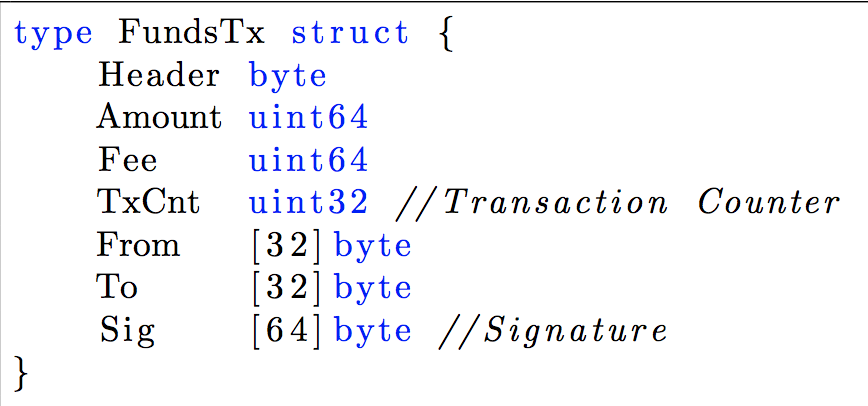
\includegraphics[width=1\textwidth]{diagrams/AccountTx_struct.png}
\caption{\label{fig:FundsTX}Structure of a FundsTx in Bazo \cite{lisg}.}
\end{figure}.


\subsection{Web NFC}
In section \ref{pocnfcbridge} the semantics of the data model of a transaction that can be shared among users in the form of a single URL was explained.
Since the support for WebNFC is limited to android devices, the functionality for writing and reading the transaction data is visible only to the users that have activated advanced options.
The corresponding UI elements are therefore hidden if the user has not activated advanced options. The same goes for browsers and devices that lack webnfc or nfc support.
Using the API for the actual read and write operations was straightforward since the API consists of one method for each of them. The data type of the NFC %??% record was set to URL.
This way the URI can be read from all types of devices. Android devices can therefore use the android system or the Bazo Wallet to scan the Tag. If the android system is used, the tag can be placed to the back of the device. If NFC is activated in the system settings and the user has unlocked the phone, the NFC record is parsed. Since the data type of the NFC record is a single URI, android's intent system is used to ask the user which application to use for the URI. This should include Google Chrome for all standard installations and the Bazo Wallet itself, if it is installed to the homescreen.


\subsection{NFC Bridge}\label{nfcbridge}
Due to limited browser support for Native API's such as webNFC, see \ref{browsersupport}, a prototype was discussed and implemented in this thesis. The prototype involved a native android application that should enable the web application to forward transaction information that could be forwarded to NFC capable devices using the Android Beam technology.
The design and requirements of such an application was outlined in \ref{pocnfcbridge} and the two main functional requirements for the application were presented.
Reading NFC messages from passive and active devices, was achieved without implementing it in the android application. This was done by changing the data model for transaction information to one that can be expressed in a single URL. With this media type, it is possible to use the tag dispatching system in android. This would work as follows:
1. An NDEF message is received when the android device is unlocked and NFC enabled.
2. The NDEF message for this application contains just one URL. Through android's intent system the application that fits best is started.
3. If the Bazo Wallet PWA was previously installed on the android device, an intent filter is present for the origin URI of the PWA. This will result in the PWA being opened with all transaction data passed as parameter.
4. If the Bazo Wallet PWA is not installed there will be no intent filter requesting the data. The user is then prompted with all applications that can handle an URI, such as a Web browser. If a browser is selected, then the Bazo payment page is opened with all transaction data passed as a parameter.
%https://developer.android.com/guide/topics/connectivity/nfc/nfc.html

Writing the transaction data to other android devices was implemented using the Android Beam technology.
The transaction data can be passed to the NFC Bridge by either manually entering it into a form or by passing it as data through an intent. Passing data to the application through parameters has the benefit that web applications can generate links that will take the user to the application. Such a link can contain further data, which would be set to the transaction data the user wants to share with another android device.
If the android phone is held against another Android Beam enabled device, the NFC Bridge application will automatically set the appropriate transaction data encoded as an NDEF message and push it to the other device.

At the time of writing, NFC support for iOS platforms was just released for their most recent publicyl available version, iOS 11. The NFC functionality offered to iOS developers covered writing and reading to NFC tags on the iPhone 7 and iPhone 7 Plus \cite{corenfc}. Thus, an NFC Bridge application similar to how it was developed for android would not extend the functionality of existing generic NFC applications. The NFC fallback capabilities with the Bazo Wallet on iOS are outlined in chapter \cite{undefined}.
\subsection{Bluetooth Low Energy}
\subsection{Quick Response Codes}
Quick Response Codes were envisioned to be the fallback way to transfer transaction data for devices that either do not support NFC or in cases where the browser does not support webNFC. With the data model explained in \cite{undefined}, all transaction data can be placed in a QR Code in the form of a single URL.
This has the intent to support devices where the browser does not allow camera access in the browser over the webRTC API \cite{undefined}. Users with such a device can still read the QR Code using a generic native application. Since all information is encoded in a single URL the payment page can be opened with all necessary information prefilled.
webRTC is a powerful new API that allows webpages to access the camera and microphone of the device. Google Chrome has supported this API for many years, therefore multiple QR Reader libraries leveraging the API exist.
On iOS devices, webRTC support has been added with the release of Safari version 11 in September 2017 \cite{safari11release}.
The QR Scanner from the coinblesk-frontend project was a simple wrapper around an existing QR Reader library. Due to the implementations in Safari 11, the underlying library had to be modified so that certain attributes were set. This allowed to run the QR Reader in the Browser of iOS devices.

\subsection{Fallback Solutions}
Subsections of chapter 4.2 outlined how existing native and web-enabled API's were leveraged for the Bazo Wallet to share transaction data. This section documents the fallback solutions that were evaluated for devices or platforms that lack the support for the API, either natively or on the web.
For android, the complete functionality of NFC could be leveraged. Writing and reading NFC tags was implemented with the web-nfc API. Complete peer to peer communication was enabled by developing an API bridge, see \ref{nfcbridge}.
As iOS platforms only support native API's when communicating over NFC and peer to peer mode is not yet included, the fallback solution to use NFC on iOS devices can be described as follows. Since all transaction data can be encoded into a single valid URL, merchants and users can transfer their transaction data to an NFC tag. This can be done with any generic NFC application or, on an android device, with the Bazo Wallet itself. iOS users can then scan the NFC tag with their preferred generic NFC application. This will open the Payment page of the Bazo Wallet, prefilled with all necessary transaction data.

\section{Blockchain Interaction}\label{blockchaininteraction}
Actual network communication with the Bazo network in a trustless way posed the most difficult technical challenge for the application. The following mechanisms had to be evaluated:

1. Building the transaction data in the schema defined in the Bazo protocol. \ref{fig:FundsTX}.
Due to technical limitations of the browser, this application context is not suitable to fullfill the requirements of a light client implementation. Reasons for this are lack of tcp communcation support, storage and data structures.
To overcome these limitations, native application wrappers for the light client written in Go were evaluated. This approach would have the advantage that each customers doesn't have to maintain a complete copy of the blockchain but transactions can be verified in trustless way. However, the current state of project that enables the mobile bindings for go did not support all networking and data structure needs to fulfill the requirement. \cite{gobind}
2. Signing the transaction data with the appropriate algorithms.
3. Verifying transaction and account information.
In order to run the Bazo Wallet as trustless as possible, the application has to maintain at least a certain amount of the blockchain to verify information. For the Bazo Wallet this would mean that the Bazo Wallet itself needs to verify blocks and transactions, or that the Bazo Wallet needs to talk with a trustworthy Bazo client. The latter approach would have been envisioned as a native application that would run on each mobile device.
The first approach was not suitable, since the lack of support for certain data types and communication protocols are present in the Browser. The latter approach could not be implemented with the given resources. However, native implementations of the Bazo Client for Android and iOS are technically feasible.

% link to gomobile, link to evaluation & future work


\subsection{Bazo Client Web interface} \label{bazoclientwebinterface}
In order to interact with the Bazo Client, a web interface had to be created. The web service was designed as a RESTful API. The following xy explains the functionality of the API.
The web service consisted of two endpoints for each type of transaction in the Bazo currency and one for the retrieval of account information such as balance and other parameters.
For each of the transaction types the following two endpoints need to be used.
\begin{itemize}
\item The endpoint at /create<Account Type>/ is used to create obtain a transaction hash given all parameters for the Transaction struct are sent. This solves the problem of lacking the appropriate data types in the browser. The  returned transaction hash can then be signed on the client.
\item The endpoint at /send<Account Type> accepts the transaction signature, which was generated on the client, and matching transaction hash. With these informations, the transaction can be considered complete, so that the underlying bazo client can distribute the transaction for further validation in the network. The web service does not validate the transaction and respond the answer to the client.
\end{itemize}  

\subsection{Transaction Signing}\label{transactionsigning}
Due to limitations of the browser for C-like structures as they would be required to create a FundsTx \ref{fig:FundsTX}, an interface had to the Bazo client had to be developed. 
The process of obtaining transaction information, requesting a new transaction, signing and dispatching it into the network is shown in figure \ref{fig:TransactionProcess}.
1. The application queries the necessary account information to request a transaction struct in a later step. This is a necessary step, since the TxCount of the transaction has to be correct in order for the transaction to be valid.
2. With the account information, the web application can send a request to the web service to create a new FundsTx struct. The Bazo client creates the appropriate structure, hashes it using the SHA3-256 algorithm and returns it to the Wallet.
3. The Wallet is now in charge of asking the user about its private key, signing the received transaction hash and sending it to the Bazo client.

This approach is comparable to the mechanism employed in the official JavaScript API of the Ripple currency \cite{ripplelib}.
Figure \ref{fig:ripplesendTx} demonstrates how a transaction can be sent with the Ripple cryptocurrency using the library. The mechanism can be outlined into the following
L1: A connection to an interface is opened over a Websocket. 
L3: A request is made to obtain relevant data and instruction for the payment.
L5: The data returned from preparing the transaction is signed.
L7: The API submits the signed Transaction over the WebSocket

Comparing the mechanism in Bazo, see Figure \ref{fig:TransactionProcess}, and Ripple, \ref{fig:ripplesendTx}, reveals certain differences, although the approach, with the respective consequences being similar.
\begin{itemize}
\item \textbf{Protocol mechanism} In Ripple, there exists a convenient method to prepare all data into a single JSON object, that needs to be signed and submitted. This step is splitted up into multiple steps in the web interface for Bazo. The client is responsible for querying the account information and then requesting a transaction hash from said information.
\item \textbf{Connection Type} Both cryptocurrencies use web interfaces for communication with a node in the Network. In Bazo http is used, while the Ripple library makes use of a WebSocket for two-way communication. Given that two-way communication is not necessary for the Bazo currency, the http approach was chosen, since this is supported by a broader range of devices and browsers.
\end{itemize}

\begin{figure}
\centering
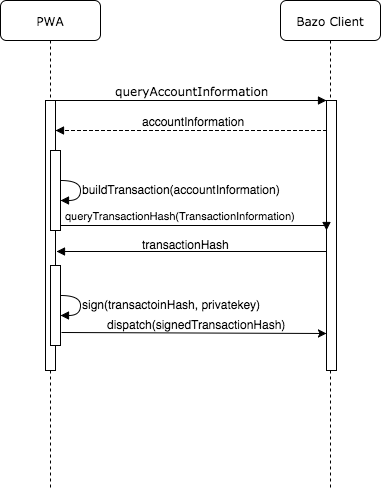
\includegraphics[width=0.7\textwidth]{diagrams/transactionProcess.png}
\caption{\label{fig:TransactionProcess}Requesting, building, signing and submitting payment information in Bazo.}
\end{figure}.

\begin{figure}
\centering
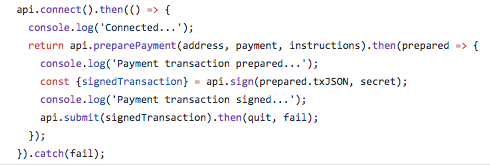
\includegraphics[width=0.7\textwidth]{diagrams/ripplelibSendTX.png}
\caption{\label{fig:ripplesendTx}Programmatically creating, signing and sending a transaction with Ripple-lib\cite{ripplelib}.}
\end{figure}.


\subsection{Client Integration}
Chapter \ref{bazoclientwebinterface} explained the interaction between the Bazo Wallet and the Bazo light client over a web interface.
This chapter explains contexts in which the bazo client can be run, consequences and documents the efforts of porting the light client to mobile devices.
Due to the security constraints one needs to be consider when interaction with other sources in a PWA, the Bazo client web interface has to be in a secure context. This would mean that an SSL certificate needs to be installed or the server needs to accessible through a secure reverse tunnel.
This makes mobile devices as a runtime unsuitable, since an SSL certificate can not easily be installed for each mobile device. However, a proof of concept was developed to show that mobile devices are technically feasible to run the client. In chapter \ref{blockchaininteraction}, it was explained that binding the bazo client that was written in the go programming language in native android development using the official tools was not possible due to a lack of support for data-types. The following xy explain how the bazo client was ported to the android operating system for ARMv5 devices.
To port the complete bazo client without any modifications to the android operating system the application was compiled  using the clang compiler. The compiler can be obtained through androids official NDK or it can be compiled from scratch. The complete toolchain was compiled targeting the arm architecture, and android API version 21 on a darwin x64bit system. The clang compiler of the toolchain was then used to configure the go environment for cross-compilation. The bazo client could then be compiled for android by configuring the golang environment for arm architectures and to use the freshly compiled clang compiler.
The binary was then copied to an android device an ran in the scope of an existing application. This is a necessary step for binaries that are run on devices were root access is not given. The application performed well, so that ngrok was used to create a secure reverse tunnel. With this in place the web application was able to interact with the bazo client running on the same device but accessible through the secure context.
This Proof of Concept could be leveraged to create an actual android application wrapping the binary. However, a solution to configure SSL appropriately would need to be found.
% reference in future work

\section{Testing}

\newpage
